\documentclass[10pt]{exam}
\usepackage[hon]{template-for-exam}
\usepackage{tikz,multicol}
\usetikzlibrary{
  calc,
  patterns,
  decorations.pathmorphing,
  decorations.markings,
  arrows,
  shapes,
  positioning,
  math,
  intersections,
  fadings
}
\usepackage{silence}
\WarningFilter{latex}{Label `question}
\WarningFilter{latex}{There were multiply-defined labels}


\title{Geometric Optics}
\author{Rohrbach}
\date{\today}

\begin{document}
\maketitle


\section*{The Ray Model of Light}

\vspace{5em}

\section*{Reflection}


\subsection*{The Law of Reflection}
  The angle of incidence is \fillin[equal][5em] to the angle of Reflection

  \vspace{3em}

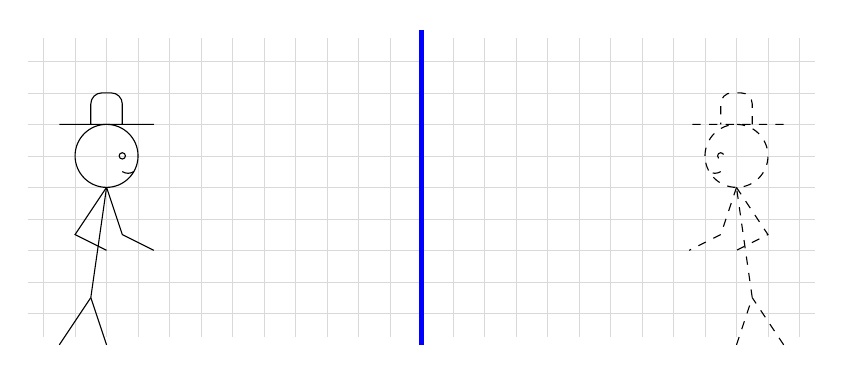
\begin{tikzpicture}
    \draw[gray!30,ultra thin] (-5,0.1) grid[step=0.4] (5,3.9);


  \def\person{
    \begin{scope}[scale=2, shift={(-2,0)}]
      \draw (0,1.2) circle (0.2);
      \coordinate (waste) at (-.1,.3);
      \coordinate (neck) at (0,1);
      \draw (waste) -- (neck);
      \draw (-.3,0) -- (waste);
      \draw (0,0) -- (waste);
      \draw (neck) -- ++(.1,-.3) -- ++(.2,-.1);
      \draw (neck) -- ++(-.2,-.3) -- ++(.2,-.1);

      \draw[rounded corners] (neck) ++(-.3,.4) -- +(.6,0)
        ++(.2,0) -- ++(0,0.2) -- ++(0.2,0) -- ++(0,-0.2);

      \path (0,1.2) ++(-30:0.2) coordinate (smile);

      \draw (neck) ++(0.1,0.2) circle (0.02)
          ++(0,-0.1) to[bend right] (smile);
    \end{scope}
  }

  \draw[ultra thick, blue] (0,4) -- (0,0);

  \begin{scope}
    \person
  \end{scope}
  \begin{scope}[xscale=-1,yscale=1, dashed]
    \person
  \end{scope}

\end{tikzpicture}

\vspace{2em}


\subsection*{Diffuse and Specular Reflection}


\vs

\subsection*{Curved Mirrors}

\begin{center}
  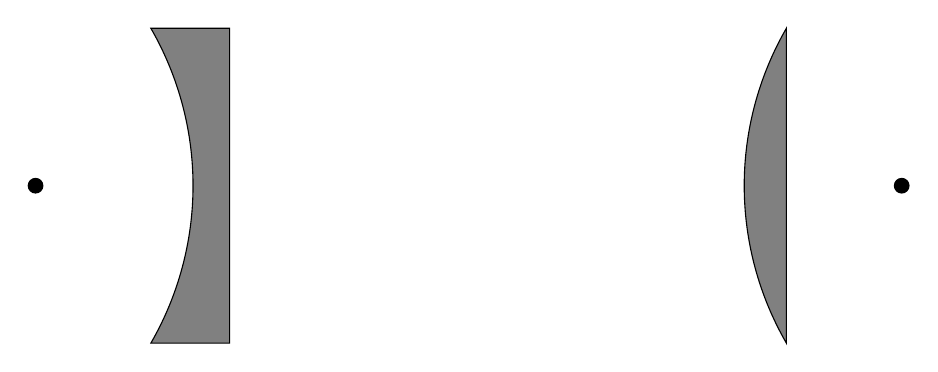
\begin{tikzpicture}

    \begin{scope}
      \def\radius{4}
      \draw[fill=gray] (\radius,0) 
        arc (0:30:\radius) --
        ++(1,0) |- (-30:\radius)
        arc (-30:0:\radius)
        -- cycle;
      %\fill[black] (0,0) circle (0.1);
      \fill[black] (0.5*\radius,0) circle (0.1);  
    \end{scope}

    \begin{scope}[shift={(15,0)}]
      \def\radius{-4}
      \draw[fill=gray] (\radius,0) 
        arc (0:30:\radius) --
        (-30:\radius)
        arc (-30:0:\radius)
        -- cycle;
      %\fill[black] (0,0) circle (0.1);
      \fill[black] (0.5*\radius,0) circle (0.1);  
    \end{scope}

  \end{tikzpicture}
\end{center}

\pagebreak

\section*{Refraction}

\vspace{10em}

\begin{itemize}
    \item when light slows down, it bends \fillin[toward][15em] normal. \vspace{2em}
  \item when light speeds up, it bends \fillin[away from][15em] normal. \vspace{3em}
\end{itemize}

\subsection*{Total Internal Reflection}

\vspace{5em}


\section*{Lenses}

\begin{center}

  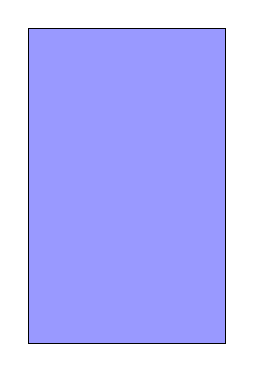
\begin{tikzpicture}
    \draw[fill=blue!40] (0,0) rectangle (2.5,4);
  \end{tikzpicture}

  \vs

  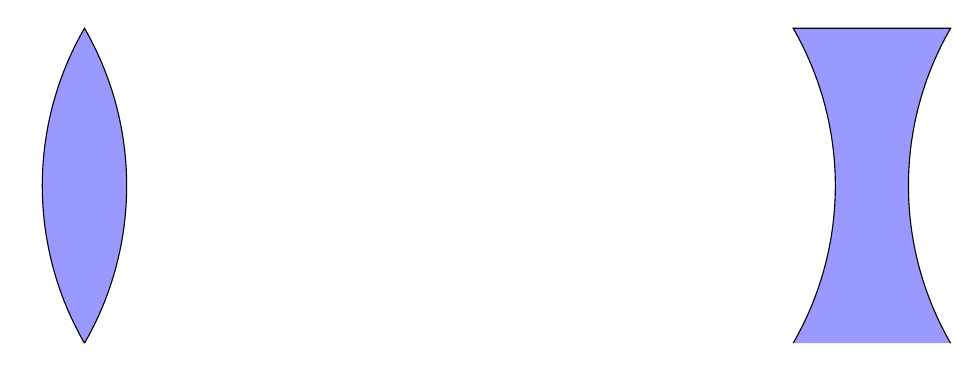
\begin{tikzpicture}
    \draw[fill=blue!40] (0,0) 
      arc (-30:30:4) 
      arc (150:210:4);
  
    \draw[fill=blue!40] (9,0) 
      arc (-30:30:4) --
      ++(2,0)
      arc (150:210:4);
  \end{tikzpicture}
\end{center}

\pagebreak


\subsection*{Refraction Practice Problems}

\begin{questions}
  \question 
    The speed of light in ice is \SI{2.29e8}{\meter\per\second}.  What is the index of refraction of ice?
    \vs

  \question
    A flashlight beam strikes the surface of a pane of glass (n=1.56) at an angle of $67^\circ$ to the normal.  What is the angle of refraction?
    \vs

  \question
    A diver shines a flashlight upward from beneath the water ($n=1.33$) at an angle $35^\circ$ to the vertical.  At what angle does the light leave the water?
    \vs

  \question
    What is the critical angle for the interface between acryllic plastic ($n=1.49$) and water ($n=1.33$).  To be internally reflected, the light must start out in which medium?
    \vs
 
\end{questions}

\pagebreak 

\section*{Images}

An image is the point where light rays \fillin[intersect][15em].

\vspace{1em}

\begin{tabular}{p{2.5in}p{0.5in}p{2.5in}}
  \textbf{virtual images} &&  \textbf{real images} \\\\
  %
  rays of light appear to intersect at a location, but in reality there is \fillin[no light][6.5em] at that location.
  %
  &&
  rays of light really do \fillin[intersect] at a point in space \\\\
  \fillin[cannot be][8em] focused on a screen &&
  \fillin[can be][8em] focused on a screen
  
\end{tabular}

\vs[3]

\subsection*{Equations for Locating Images}


\vs[2]

\subsection*{Sign Conventions}

\renewcommand{\arraystretch}{2}

\begin{tabular}{cll}
$d_o$ & distance between mirror/lens and object \\
$d_i$ & distance between mirror/lens and image \\
$f$   & focal length \\ 
$h_o$ & height of object \\
$h_i$ & height of image \\
$m$   & magnification \\
\end{tabular}





\pagebreak


\section*{Image Formation in Mirrors}

\paragraph{Three (Four?) Principle Rays} \hfill
\begin{enumerate}
  \item A ray travelling parallel to the principal axis gets reflected to \fillin[the focal point][10em]
  \item A ray traveling through the focal point gets reflected  \fillin[parallel to the axis][10em]
  \item A ray that goes through center of curvature gets reflected \fillin[along itself][10em]
  \item A ray that hits the precise center of the mirror gets reflected \fillin[at the same angle across the normal][15em]

\end{enumerate}

\vs

\paragraph{Example \#1}\hfill

\noindent
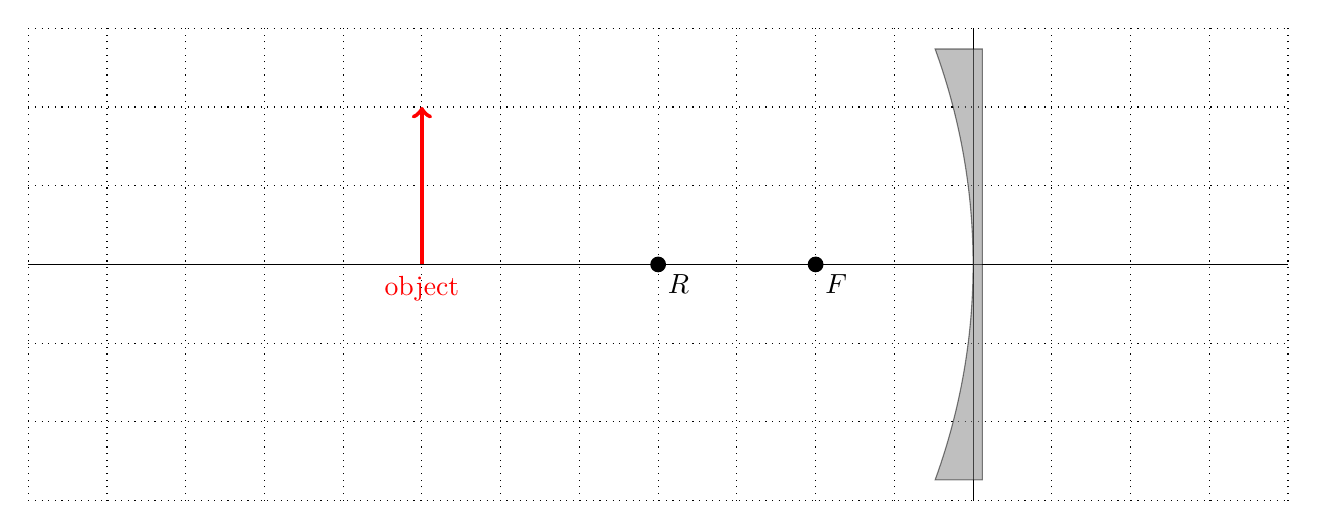
\begin{tikzpicture}
  \def\objloc{-3}
  \def\objheight{2}


  \draw[dotted,thin] (-8,-3) grid (8,3);
  \draw (-8,0) -- (8,0);
  \draw (4,-3) -- (4,3);


  \begin{scope}[shift={(-4,0)}]
    \def\radius{8}
    \draw[fill=gray,semitransparent] (\radius,0) 
      arc (0:20:\radius) --
      ++(0.6,0) |- (-20:\radius)
      arc (-20:0:\radius)
      -- cycle;  
  \end{scope}

  \fill[black] (0,0) circle (0.1) 
    node[below right] {$R$};
  \fill[black] (2,0) circle (0.1)
    node[below right] {$F$};

  \draw[ultra thick, red, ->] (\objloc,0)
    node[below] {object}
      -- ++(0,\objheight);


\end{tikzpicture}

\vs

\pagebreak

\paragraph{Example \#2}\hfill

\noindent
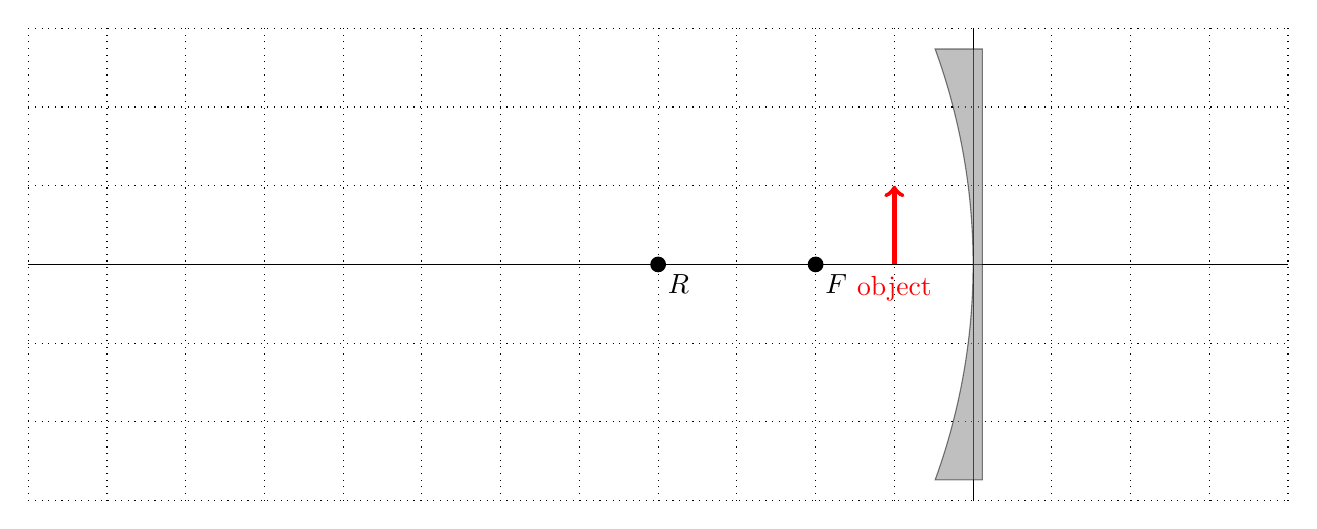
\begin{tikzpicture}
  \def\objloc{3}
  \def\objheight{1}

  \draw[dotted,thin] (-8,-3) grid (8,3);
  \draw (-8,0) -- (8,0);
  \draw (4,-3) -- (4,3);


  \begin{scope}[shift={(-4,0)}]
    \def\radius{8}
    \draw[fill=gray,semitransparent] (\radius,0) 
      arc (0:20:\radius) --
      ++(0.6,0) |- (-20:\radius)
      arc (-20:0:\radius)
      -- cycle;  
  \end{scope}

  \fill[black] (0,0) circle (0.1) 
    node[below right] {$R$};
  \fill[black] (2,0) circle (0.1)
    node[below right] {$F$};

  \draw[ultra thick, red, ->] (\objloc,0)
    node[below] {object}
      -- ++(0,\objheight);


\end{tikzpicture}

\vs

\paragraph{Example \#3}\hfill

\noindent
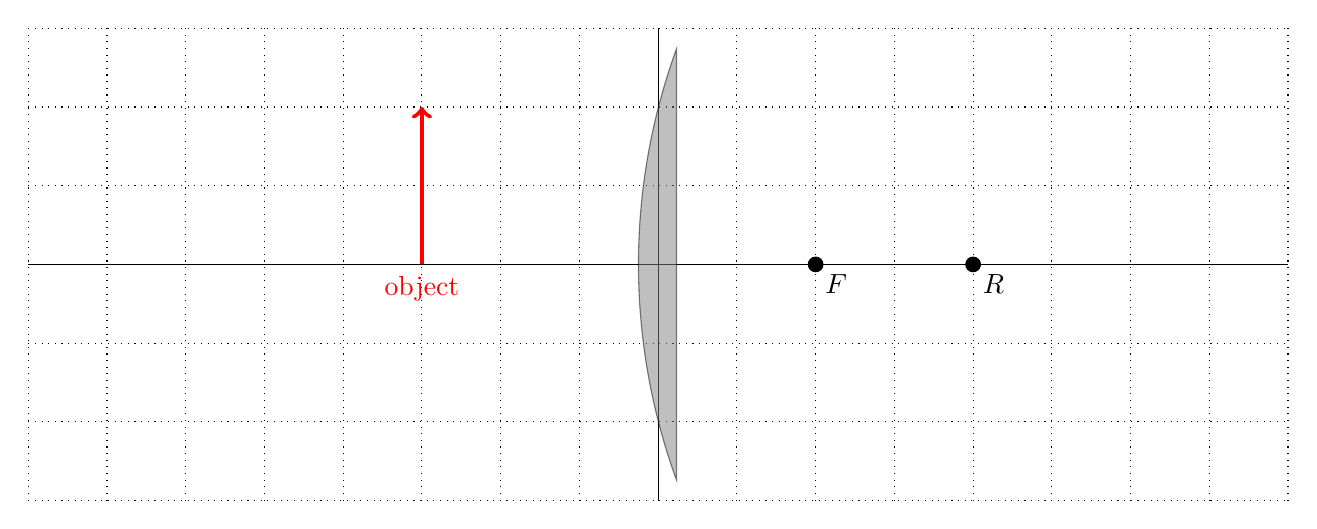
\begin{tikzpicture}
  \def\objloc{-3}
  \def\objheight{2}

  \draw[dotted,thin] (-8,-3) grid (8,3);
  \draw (-8,0) -- (8,0);
  \draw (0,-3) -- (0,3);


  \begin{scope}[shift={(7.75,0)}]
    \def\radius{8}
    \draw[fill=gray,semitransparent] (-\radius,0) 
      arc (180:160:\radius)
      -- (200:\radius)
      arc (200:180:\radius)
      -- cycle;  
  \end{scope}

  \fill[black] (4,0) circle (0.1) 
    node[below right] {$R$};
  \fill[black] (2,0) circle (0.1)
    node[below right] {$F$};

  \draw[ultra thick, red, ->] (\objloc,0)
    node[below] {object}
      -- ++(0,\objheight);


\end{tikzpicture}

\vs


\pagebreak

\section*{Image Formation in Lenses}

\paragraph{Three Principle Rays} \hfill
\begin{enumerate}
  \item A ray travelling parallel to the principal axis gets refracted to \fillin[the focal point][10em]
  \item A ray traveling through the focal point gets refracted  \fillin[parallel to the axis][10em]
  \item A ray that goes through center of optical center \fillin[does not refract][10em]
\end{enumerate}

\paragraph{Example \#1}\hfill

\noindent
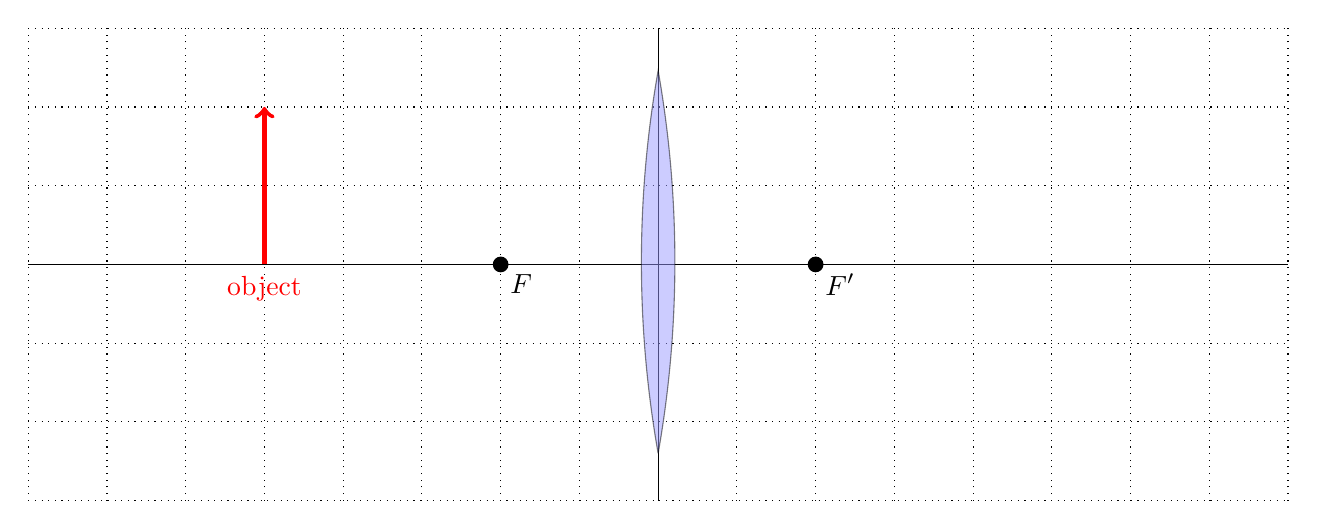
\begin{tikzpicture}
  \def\objloc{-5}
  \def\objheight{2}


  \draw[dotted,thin] (-8,-3) grid (8,3);
  \draw (-8,0) -- (8,0);
  \draw (0,-3) -- (0,3);
  \fill[black] (-2,0) circle (0.1) 
    node[below right] {$F$};
  \fill[black] (2,0) circle (0.1)
    node[below right] {$F'$};

  \draw[fill=blue!40,semitransparent] (0,-2.4) 
    arc (-10:10:14) 
    arc (170:190:14);



  \draw[ultra thick, red, ->] (\objloc,0)
    node[below] {object}
      -- ++(0,\objheight);


\end{tikzpicture}

\vs

\paragraph{Example \#2}\hfill

\noindent
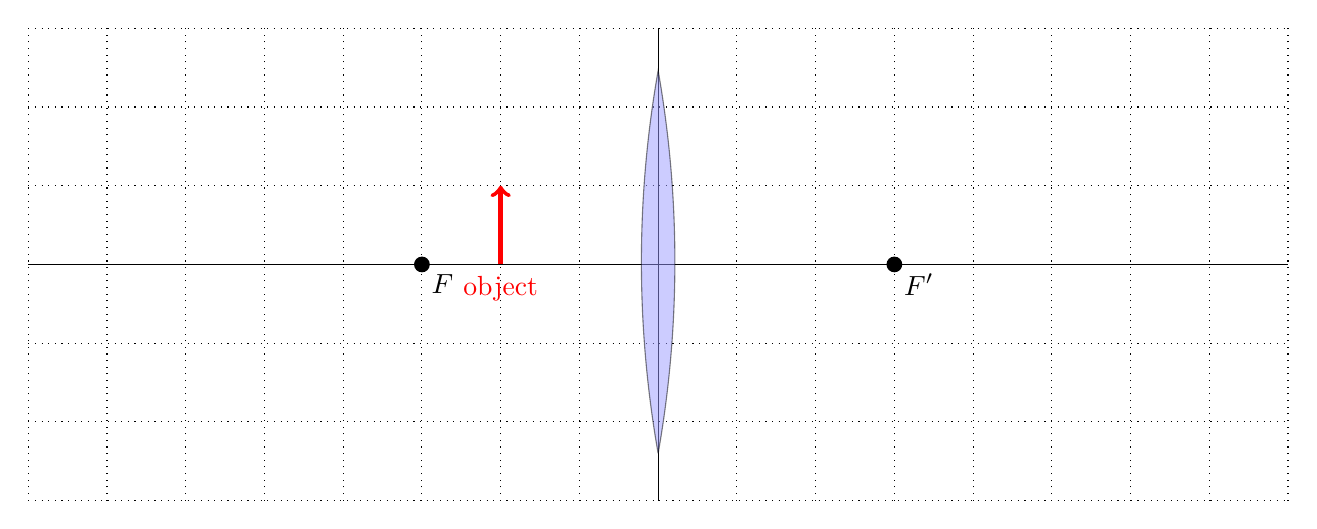
\begin{tikzpicture}
  \def\objloc{-2}
  \def\objheight{1}
  \def\focal{3}


  \draw[dotted,thin] (-8,-3) grid (8,3);
  \draw (-8,0) -- (8,0);
  \draw (0,-3) -- (0,3);
  \fill[black] (-\focal,0) circle (0.1) 
    node[below right] {$F$};
  \fill[black] (\focal,0) circle (0.1)
    node[below right] {$F'$};

  \draw[fill=blue!40,semitransparent] (0,-2.4) 
    arc (-10:10:14) 
    arc (170:190:14);



  \draw[ultra thick, red, ->] (\objloc,0)
    node[below] {object}
      -- ++(0,\objheight);


\end{tikzpicture}

\vs

\pagebreak

\paragraph{Example \#3}\hfill

\noindent
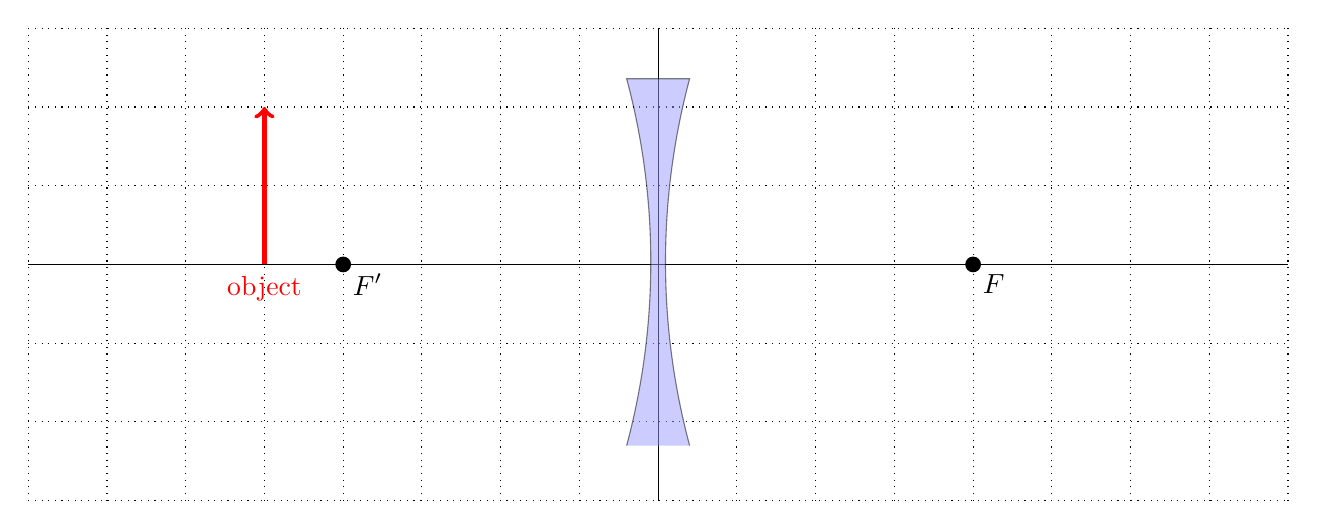
\begin{tikzpicture}
  \def\objloc{-5}
  \def\objheight{2}
  \def\focal{-4}


  \draw[dotted,thin] (-8,-3) grid (8,3);
  \draw (-8,0) -- (8,0);
  \draw (0,-3) -- (0,3);
  \fill[black] (-\focal,0) circle (0.1) 
    node[below right] {$F$};
  \fill[black] (\focal,0) circle (0.1)
    node[below right] {$F'$};

  \draw[fill=blue!40,semitransparent] (-0.4,-2.3) 
    arc (-15:15:9) --
    ++(.8,0)
    arc (165:195:9);



  \draw[ultra thick, red, ->] (\objloc,0)
    node[below] {object}
      -- ++(0,\objheight);


\end{tikzpicture}

\vs[2]

\subsection*{Lens Equation Practice Problems}

\begin{questions}
  \question
    A rutabaga, which has a height of 44~cm is placed 10~cm in front of a converging lens.  The image produced has a height of 66~cm and is \emph{inverted}.  

    \begin{parts}
      \part What is the image distance?
      \part What is the power of the lens?
    \end{parts}
    \vs

  \question
    A diverging lens has a focal length of 9.0~cm, and an object is placed 3.0~cm from the lens.

    \begin{parts}
      \part What would be the distance of the image from the lens?
      \part What is the magnification of the image?
      \part Will the image be real or virtual, upright or inverted?  How do you know?
      \part What is the power of the lens?
    \end{parts}
    \vs

  \question
    A lens has a power of 0.1 Diopters.  Locate the image of an antelope placed upright 30.0 m from the lens.  Find the magnification of the image.  
    \vs

\end{questions}

\end{document}